\section{Color-Adaptive Decomposition}

In this section, we present methods for more efficient decomposition from color-volume to binary-volume, efficiency here refering to the number of binary depth planes that are used to represent a color depth plane. 

\subsection{Motivation}
In the method presented in Sec. \todo{find the section number}, each color voxel was decomposed into the nearest 24 binary depth planes. Since our display's LEDs can change color and intensity over a very large range on a per-binary frame basis, we don't need to limit our display to a fixed pattern of LED colors and intensities or to 8 bits-per-color. A more optimum decomposition method might use fewer number of binary voxels to represent the same color voxel. It is useful to reduce the number of binary voxels that represent each color voxel for the following reasons:

\begin{enumerate}
    \item This will reduce the depth-blur associated with each color voxel.
    \item This may be useful for more compact prototypes because the more compact DMD projectors have a slower refresh rate than the DMD projector used in our display.
    \item We may be able to achieve High Dynamic Range imagery.
    \item With fewer number of binary voxels representing each color voxel, we can represent objects that are transparent and closer to each other than with the fixed pipeline decomposition. With the fixed pipeline decomposition, we can not represent objects along the same depth that are closer than $3 \times \text{color bit-depth}$.
\end{enumerate}

\subsection{Approach}
The basic idea behind the color adaptive decomposition methods explored here is that of error propagation or diffusion. 
Starting at the nearest depth plane, we consider the slice of the color volume and do the best of representing it with a binary image and an arbitrary LED color. 
Unavoidably, there will be errors, which are propagated onto the next depth plane. 
At the next depth plane, the current depth's slice of the color volume and the propagated errors are added and considered as the target image for the decomposition.
The pseudo-code for this approach is given in Algorithm.~\ref{alg:colorAdaptiveMethodOne}.

Let $R$ denote residue, $T$ denote the target image, $A$ denote the actual reconstruction, $L$ denote the LEDs, $B$ denote the binary image, and $V$ denote the volume. Then, 

\begin{algorithm}
    \caption{Outline of error propagation appoach}
    \label{alg:colorAdaptiveMethodOne}
    \hspace*{\algorithmicindent}\textbf{Input:} $V$\\
    \hspace*{\algorithmicindent}\textbf{Output:} $B, L$
    \begin{algorithmic}[1]
        \STATE{$R \gets \text{zeros}$}
        \FOR{$d \gets 1$ \TO $\numPlanes$}
        \STATE{$I \gets V \lbrack :,:,d \rbrack $}
        \STATE{$T \gets I + R$}
        \STATE{${(B_d,L_d)} \gets \text{Decompose$(T)$}$}
        \STATE{$R \gets T - \text{Reconstruct$(B_d, L_d)$}$}
        \ENDFOR
    \end{algorithmic}
\end{algorithm}

The methods explored here differ from each other in the way the target image at each depth is decomposed, i.e., the \emph{Decompose} function in Algorithm.~\ref{alg:colorAdaptiveMethodOne}.
In the sections below, we explore some possible ways to decompose the target image at each depth.
For each of the methods below, the decomposition step tries to minimize the L2-norm between the decomposition and the target images:
\begin{equation}
    \argmin_{B_d,L_d} ||T - \text{Reconstruct}(B_d, L_d) ||^2
\end{equation}

However, the problem with trying to decompose a 24-bit target RGB image into a 1-bit DMD image and an RGB LED value is that:
\begin{enumerate}
    \item Because the DMD pattern is common for the three color channels, the decomposition is not separable among the color-channels, e.g., a particular DMD pattern may have very low loss for the red channel but very high for the green channel such that the combined error might be lesser than completely leaving out green channel. 
    \item Something to do with binarization. The threshold determines whether you under-expose or over-expose. When you under-expose, the errors are propagated much farther away from the slice which caused the error.
    \item 
\end{enumerate}

\subsubsection{Brute-force}
In this method, we calculate the decomposition for every combination of color channel. These are the difference combinations of color channels: $O_1 = $\{ R, 0, 0 \}, $O_2 = $ \{ 0, G, 0 \}, $O_3 = $ \{ 0, 0, B \}, $O_4 = $ \{ R, B, 0 \}, $O_5 = $ \{ R, 0, B \}, $O_6 = $ \{ 0, G, B \}, $O_7 = $ \{ R, G, B \}, where 0 in the tuple simply indicates that that color channel is not considered in that option for the 

\begin{algorithm}
    \caption{Brute-force color decomposition}
    \label{alg:bruteforce}
    \hspace*{\algorithmicindent}\textbf{Input:} $T$\\
    \hspace*{\algorithmicindent}\textbf{Output:} $B, L$
    \begin{algorithmic}[1]
        \STATE{$R \gets \text{zeros}$}
        \FOR{$i \gets 1$ \TO $7$}
        \STATE{$(R,G,B) = \text{split}(T)$}
        \STATE{$R = O_i[1] R$}
        \STATE{$I \gets V \lbrack :,:,d \rbrack $}
        \STATE{$T \gets I + R$}
        \STATE{${(B_d,L_d)} \gets \text{Decompose$(T)$}$}
        \STATE{$R \gets T - \text{Reconstruct$(B_d, L_d)$}$}
        \ENDFOR
    \end{algorithmic}
\end{algorithm}

\subsubsection{Highest Energy Channel Minimization}

\subsubsection{Projected Gradient}

\subsection{Evaluation}
visual quality

number of binary voxels

transparencies

PSNR of focal stacks

SSIM of focal stacks

\subsection{Results}
\begin{figure}[h!]
\centering
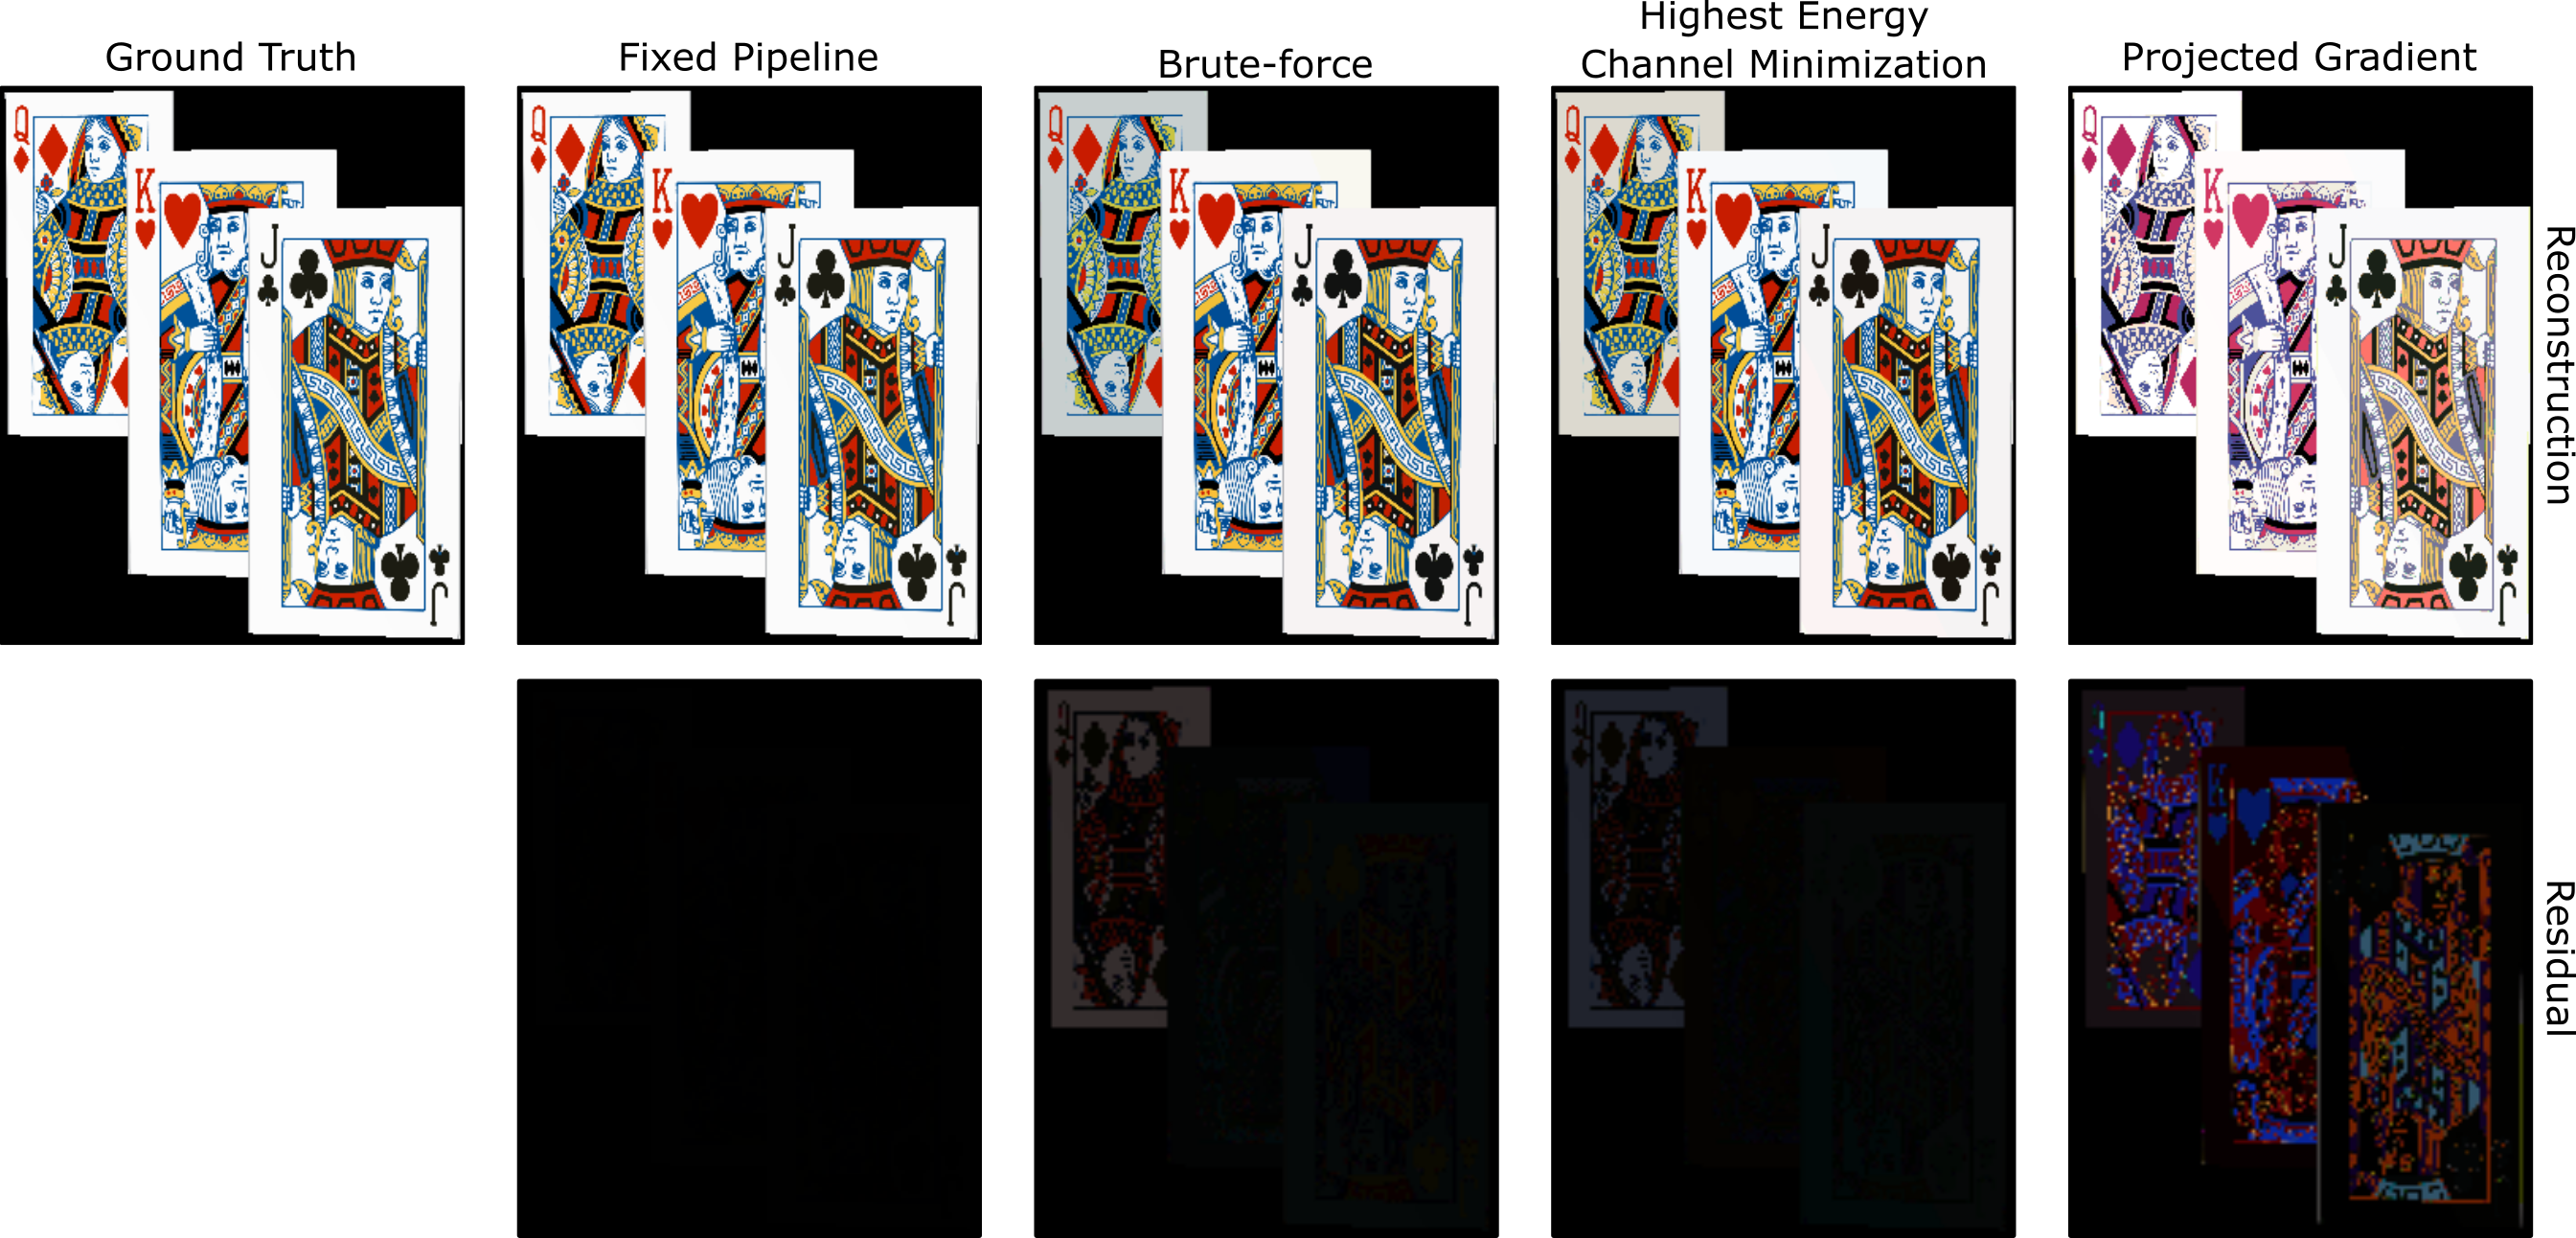
\includegraphics[width=0.99\columnwidth]{images/volumetric/cad_results/cad_visual_quality}
\caption[Color Adaptive Decomposition: visual quality]{Simulation results showing visual quality for the different color adaptive decomposition algorithms.}
\label{fig:volumetric:cad:visual_quality}
\end{figure}


\begin{figure}[h!]
\centering
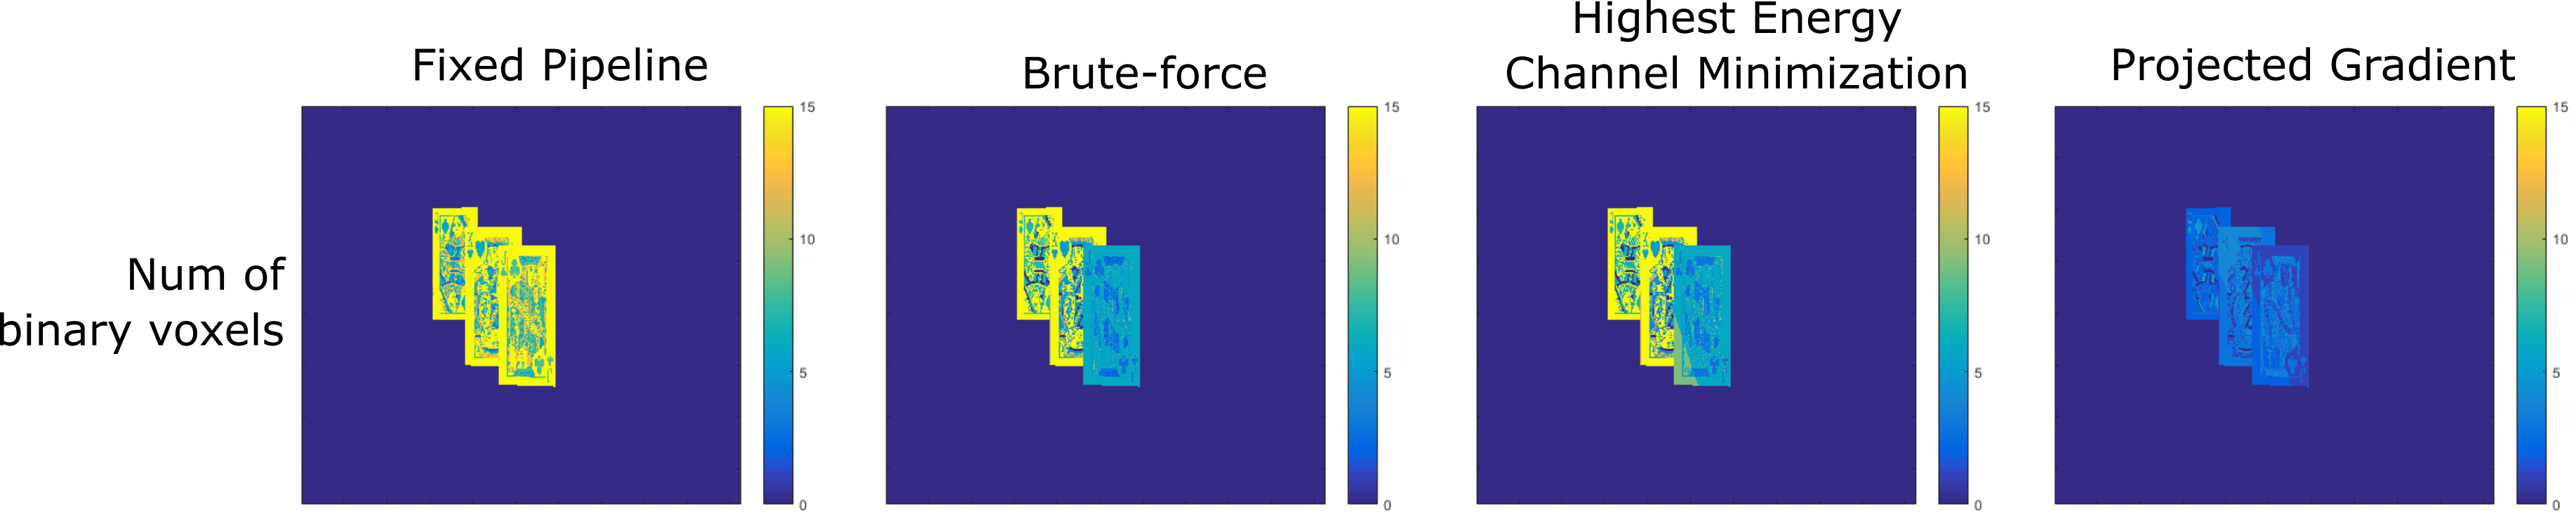
\includegraphics[width=0.99\columnwidth]{images/volumetric/cad_results/cad_num_binary_voxels}
\caption[Color Adaptive Decomposition: number of binary voxels]{Simulation results showing the number of binary voxels needed to represent a color voxel for the different color adaptive decomposition algorithms.}
\label{fig:volumetric:cad:num_binary_voxels}
\end{figure}


Fig.~\todo{rename} compares the number of binary voxels needed to present each color voxel for the different algorithms above. Fig.~\todo{rename} compares the reconstructed image quality and residual images for the different algorithms above. Note that while the \emph{Fixed pipeline} approach gives the best visual quality, the \emph{Projected gradient} approach gives the least number of binary voxels needed to present each color voxel. The \emph{Fixed pipeline} approach gives a residual of zero because it is a deterministic algorithm where the binary volume is guaranteed to fully represent the color volume.

\subsection{Future Work}
\todo{Polish up these things} Above approaches are slow. Opportunity to apply Deep Neural Networks. Global optimization is another direction.
